% paper proposal for the Modelica 2017 Conference

%%% By default the modelica LaTeX class uses bibtex and natbib for refrences
\documentclass{resources/modelica}
%%% As alternative also for unicode and @online support
%%% use the more modern biber and biblatex instead
%\documentclass[backend=biber]{modelica}
%\addbibresource{example-paper.bib}
%\usepackage[utf8]{luainputenc} % utf8 input encoding that should work for both pdflatex and lualatex, but might not be available in every installation
\usepackage[utf8]{inputenc} % utf8 input encoding which should work with pdflatex, but not lualatex

\hypersetup{%
	pdftitle  = {Towards a Standard-Conform, Platform-Generic and Feature-Rich Modelica Device Drivers Library},
	pdfauthor = {Bernhard Thiele, Thomas Beutlich, Volker Waurich, Martin Sjölund,
	Tobias Bellmann}, pdfsubject = {12th International Modelica Conference 2017},
  pdfkeywords = {Modelica, embedded systems, real-time simulation},
	colorlinks,
	linkcolor=black,
	urlcolor=black,
	citecolor=black,
	pdfpagelayout = SinglePage,
	pdfcreator = pdflatex,
	pdfproducer = pdflatex}

\newcommand{\modelica}[1]{\lstinline[language=modelica]|#1|}
\newcommand{\BTHI}[1]{{\color{blue}{$\parallel_\textrm{BTHI}$#1$\parallel$}}}
\newcommand{\TBEU}[1]{{\color{orange}{$\parallel_\textrm{TBEU}$#1$\parallel$}}}
\newcommand{\VWAU}[1]{{\color{red}{$\parallel_\textrm{VWAU}$#1$\parallel$}}}
\newcommand{\MSJO}[1]{{\color{green}{$\parallel_\textrm{MSJO}$#1$\parallel$}}}
\newcommand{\TBEL}[1]{{\color{magenta}{$\parallel_\textrm{TBEL}$#1$\parallel$}}}



% begin the document
\begin{document}
\thispagestyle{empty}

\title{Towards a Standard-Conform, Platform-Generic and Feature-Rich Modelica Device Drivers Library}
\author[1]{Bernhard Thiele}
\author[2]{Thomas Beutlich}
\author[3]{Volker Waurich}
\author[1]{Martin Sjölund}
\author[4]{Tobias Bellmann}
\affil[1]{PELAB, Linköping University, Sweden,
{\small\texttt{\{bernhard.thiele,martin.sjoelund\}@liu.se}}}
\affil[2]{ESI ITI GmbH, Germany, {\small\texttt{thomas.beutlich@esi-group.com}}}
\affil[4]{Institute of System Dynamics and Control, DLR, Germany, {\small\texttt{tobias.bellmann@dlr.se}}}


\date{} % <--- leave date empty
\maketitle\thispagestyle{empty} %% <-- you need this for the first page
\abstract{%
There are many cases there simulation applications need to interact with their
environment. Typical examples are Human-in-the-Loop (HITL) simulators (including
flight, driving, and marine training simulators), Hardware-in-the-Loop (HIL)
simulators, but also offline process simulators which cannot operate in a
completely self-contained manner and therefore need to be coupled to external
applications. Embedded control applications are another related area which
requires that applications interact with their environment. The
\emph{Modelica\_DeviceDrivers} library, which had its first release as
open-source library in 2012, tries to cater for such use cases. This paper
describes the library for the first time and reports about the numerous
challenges that the project experienced to meet its goal of supporting several
platforms and tools within a standard-conform, platform-generic, feature-rich,
and easy-to-use Modelica library.}

\noindent\emph{Keywords: HITL, HIL, real-time, embedded control applications,
external C}

\section{Introduction}
\BTHI{TODO: Bernhard, Tobias}\\

The most common usage of Modelica models is for offline simulation experiments.
However, in many cases simulations need to interact with their environment.
Typical examples are Human-in-the-Loop (HITL) simulators (including flight,
driving, and marine training simulators), Hardware-in-the-Loop (HIL) simulators,
but also offline process simulators which cannot operate in a completely
self-contained manner and therefore need to be coupled to external applications.
Furthermore, Modelica can be used for developing (model-based) control
applications which also require interaction with their environment.

There are different approaches for enabling the above mentioned applications in
the context of Modelica. Several development environments offer tool
chains for real-time simulation and/or model-based development of embedded
control applications. Some of these environments can be coupled with Modelica
tools, \textit{e.g.}, by wrapping code which is generated from Modelica tools
into respective tool internal representations which can be connected to hardware
devices in the respective development environment.

The \emph{Modelica\_DeviceDrivers} (MDD) library uses a different approach.
The MDD library provides access to external devices by utilizing Modelica's external
function interface for interfacing to the C API of various device drivers directly from Modelica
models (see Section~\ref{ModelicaDeviceDrivers}).

Historically, the origins of the MDD library can be traced back to the
\emph{ExternalDevices} library \citep{Bellmann2009}\ldots
\BTHI{TODO: Bernhard, Tobias , \cite{Elmqvist2009}}


\section{Modelica\_DeviceDrivers}
\label{ModelicaDeviceDrivers}
\BTHI{TODO: Bernhard, Thomas, Volker}

The MDD library allows to access hardware devices from Modelica models.
This is achieved by using the Modelica external C interface to call the
appropriate C driver functions provided by the underlying operating system (see
Section~\ref{sec:CrossPlatformSupport}).

The library is organized in several layers as indicated in
Figure~\ref{fig:MDDLayeredArchitecture}. Notice that the library
provides two high-level Drag \& Drop block interfaces. The first (\texttt{.Blocks}) is
compatible to Modelica 3.2, using the traditional \modelica{when sample()}
element for periodically calling Modelica functions from the \textsf{Function Layer}. The second
(\texttt{.ClockedBlocks}) uses the synchronous language elements extension
introduced in Modelica 3.3 and is compatible with the
Modelica\_Synchronous library \citep{Otter2012}. Due to this support the MDD
library formally depends on the Modelica\_Synchronous library, but in
practice the Modelica\_Synchronous library (and tool support for the
synchronous language elements extension) is only required if one actually wants
to use the clocked block interface.
\begin{figure}[htb]
\begin{center}
  \includegraphics[width=\columnwidth]{figures/MDDLayeredArchitecture}
  \caption{MDD layered architecture.}
  \label{fig:MDDLayeredArchitecture}
\end{center}
\end{figure}

\subsection{Cross-Platform Support}
\label{sec:CrossPlatformSupport}

Currently MS Windows and Linux are supported as main platforms, but recent
prototypical work also targets popular embedded systems boards directly (see
Section~\ref{sec:EmbeddedControl}).



\subsection{Enhanced Tool Support}
\subsection{Library Structure}
\subsection{Interfaces}

\subsection{Features}

Features (aide-mémoire):
\begin{itemize}
  \item SerialPackager
  \item Communication
    \begin{itemize}
      \item UDP
      \item Shared Memory
      \item Softing CAN and Socket CAN
      \item RS232
    \end{itemize}
  \item input devices
    \begin{itemize}
      \item keyboard
      \item joystick/gamepad
      \item 3Dconnexion Spacemouse.
    \end{itemize}
  \item Operating System
    \begin{itemize}
      \item Realtime Synchronization
      \item Random numbers
    \end{itemize}
  \item Hardware I/O
    \begin{itemize}
      \item Comedi
    \end{itemize}
\end{itemize}


\noindent  New features:
\begin{itemize}
  \item Big endian
  \item Serial port on Win
  \item TCP/IP client
  \item LCM / UDP Broadcast
  \item Bluetooth
  \item MQTT
  \item \ldots
\end{itemize}

\section{Modelica Standard Compliance}
\BTHI{TODO: Thomas, Bernhard}

\subsection{Enhancements}

\subsection{Pitfalls and Open Issues}

Aide-mémoire:
\begin{itemize}
  \item Serialpackager
  \item Automatic buffer size
  \item External objects in equation
  \item Construction of external objects in record
  \item Linking to platform-dependent system libraries
  \item Missing fixed attribute for String
  \item Support of several include directories
\end{itemize}

\section{Applications}

\subsection{Arduino}
\BTHI{TODO: Volker}

The arduino is an open-source electronics platform which makes it very easy to read sensors, process the data and send it to another device via a serial connection \citep{arduino:2016}.
With the help of Modelica Device Drivers serial port implementation, the arduino can be utilized to make sensor data available in a real-time Modelica model.
Using different kinds of potentiometers, it is possible to build customized control devices.
As an exemplary application, pedals for a driving simulator can be equipped with a rotary potentiometer in order to measure the displacement.
This data can be send via a serial connection to a \textit{Blocks.Comunication.SerialPortReceive} in order to drive a virtual vehicle.
Hence, expensive or unavailable input devices can be substituted by self-built constructions.
By using a bluetooth module, a wireless connection between arduino and the simulator is set up easily.
\VWAU{I could add arduino code or an arduino circuit diagram here.}

\subsection{Arduino, Raspberry PI, embedded control}
\label{sec:EmbeddedControl}
\BTHI{TODO: Bernhard, Martin}

\subsection{HID Joystick}
\BTHI{TODO: Volker }

\subsection{DLR Demonstrators}
\BTHI{TODO: Tobias}

\section{Outlook}
\BTHI{TODO: Bernhard, Thomas, Volker}

\section*{Acknowledgements}


%%% choose one of the following: %%%
%% References using bibtex (default)
\bibliography{modelica2017_Modelica_DeviceDrivers}

%% References using biber and biblatex
%\printbibliography

\end{document}
